\documentclass[9pt]{beamer}
\usetheme{polimi}


\usepackage{amsmath}
\usepackage{amssymb}
\usepackage{bm} % For bold math symbols
\usepackage{graphicx}
\usepackage{tikz}
\usetikzlibrary{positioning}



\usepackage{subfig} % Changed from subfigure (deprecated)
\usepackage{multirow}
\usepackage{multicol}
\usepackage{color}
\definecolor{darkblue}{rgb}{0.12, 0.47, 0.71}
\definecolor{darkorange}{rgb}{1.0, 0.50, 0.05}
\definecolor{darkgreen}{rgb}{0.17, 0.63, 0.17}
\definecolor{darkred}{rgb}{0.84, 0.15, 0.16}
\usepackage{url}
\usepackage{hyperref}
\usepackage{listings}
\usepackage[noend]{algorithm}
\usepackage{physics} 
% add image path
\graphicspath{{../Images/}}

% bibliography
\usepackage[backend=biber,style=alphabetic,sorting=none]{biblatex}
\addbibresource{mimesis.bib}


\newcommand{\supervisors}[2]{
  
    \hspace{-0.8em}
  \begin{tabular}{ll}
  \small Advisor: & \small #1 \\
  \small Co-advisor: & \small #2
  \end{tabular}
}



\DeclareMathOperator{\argmin}{argmin}
\DeclareMathOperator{\argmax}{argmax}





\title{A Modified Neural Modes Framework for\\ Soft Tissue Simulation}
\author{Andrea Bonifacio }
\date{AY: 2024-2025  \vspace{-5em} \hspace{2cm} \supervisors{Prof. Stefano Pagani}{Dr. Stéphane Cotin}
}

\begin{document}

\begin{frame}
\titlepage
\end{frame}

\begin{frame}{The problem: Soft Tissue Simulation}
    \begin{columns}[T]
        \begin{column}{0.6\textwidth}
            \begin{itemize}
                \item Soft tissue simulation is crucial in medical applications, such as computer-assisted surgery.
                \item High-fidelity, like Finite Elements Method (FEM) simulations are computationally expensive, making real-time applications challenging.
                \item There is a strong need for fast, accurate methods that can handle large, nonlinear deformations.
            \end{itemize}
        \end{column}
        \begin{column}{0.4\textwidth}
            \begin{figure}
                \centering
                    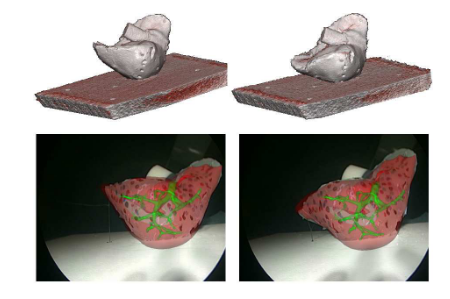
\includegraphics[width=\textwidth]{Images/liver_2.png}
                    \caption{Digital twin of a liver undergoing a deformation during computer-assisted surgery. Figure from \cite{Haouchine_Dequidt_Peterlik_Kerrien_Berger_Cotin_2013}.}
            \end{figure}
        \end{column}
    \end{columns}
\end{frame}

\begin{frame}{Related Work}
    \begin{itemize}
        \item \textbf{MeshGraphNet} \cite{pfaffLearningMeshBasedSimulation2021a} and similar deep learning models have demonstrated impressive speedups in physical simulations.
        \item However, these models are often \textbf{black-box} in nature, and they tend to \textbf{accumulate errors} over time, leading to inaccuracies in long-term simulations.
        \item  We take inspiration from the \textbf{Neural Modes} paper \cite{Wang_Du_Coros_Thomaszewski_2024}, which tries to address these issues.
    \end{itemize}
\end{frame}


\begin{frame}{Computational Mechanics Notation}
    \begin{block}{Kinematics of Deformation}
        \begin{itemize}
            \item \(\bm{X}\): Position of a material point in the \textbf{reference configuration}.
            \item \(\bm{x}(\bm{X}, t)\): Position of the same point in the \textbf{current configuration} at time \(t\).
            \item \(\bm{u}(\bm{X}, t)\): \textbf{Displacement vector}, defined as:
            \(
                \bm{u}(\bm{X}, t) = \bm{x}(\bm{X}, t) - \bm{X}.
            \)
        \end{itemize}
    \end{block}
    
    \begin{block}{Deformation Gradient}
        \[
            \bm{F} = \frac{\partial \bm{x}}{\partial \bm{X}} = \bm{I} + \nabla_{\bm{X}} \bm{u},
        \]
        where:
        \begin{itemize}
            \item \(\bm{F}\): Deformation gradient tensor.
            \item \(\bm{I}\): Identity tensor.
            \item \(\nabla_{\bm{X}} \bm{u}\): Gradient of the displacement field.
        \end{itemize}
    \end{block}
\end{frame}

\begin{frame}{Neo-Hookean Model}
    \begin{columns}[T]
        \begin{column}{0.5\textwidth}
            \textbf{Neo-Hookean Hyperelasticity}
                The strain-energy density function $\Psi$ is:
                \[
\begin{split}
                        \Psi(\bm{F}) = \frac{\mu}{2} (I_C - 3 - 2\ln(J))\\ + \frac{\lambda}{4} (J^2 - 1 - 2\ln(J)),
\end{split}                \]
                where:
                \begin{itemize}
                    \item \(\mu, \lambda\): Material parameters.
                    \item \(J = \det(\bm{F})\): Volume change.
                \end{itemize}
                We define the first Piola-Kirchhoff stress tensor \(\bm{P}\) as:
                \[
                    \bm{P} = \frac{\partial \Psi}{\partial \bm{F}} 
                \]
        \end{column}
        \begin{column}{0.5\textwidth}
            \textbf{Static Problem}
                The static equilibrium of the object is described by the following system of PDEs, which represents the full-order model:
                \begin{equation}
                    \begin{cases}
                        - \nabla_X \cdot \bm{P} = \bm{b} \quad \text{in} \quad \Omega, \\
                        \bm{u} = \bm{u}_D \quad \text{on} \quad \Gamma_D, \\
                        \bm{P} \cdot \bm{N} = \bm{t} \quad \text{on} \quad \Gamma_N.
                    \end{cases}
                    \label{eq:static_problem}
                \end{equation}
                where:
                \begin{itemize}
                    \item \(\bm{b}\): Body forces.
                    \item \(\Gamma_D, \Gamma_N\): Boundary conditions.
                \end{itemize}
        \end{column}
    \end{columns}
\end{frame}

% \begin{frame}{Neo-Hookean Model}    
%     \begin{block}{Equation of Motion}
%         The dynamic behavior of the object is governed by the following system of PDEs, which represents the full-order model. Solving this system is accurate but computationally expensive.
%         \begin{equation}
%             \begin{cases}
%                 \rho \frac{\partial^2 \bm{u}}{\partial t^2} - \nabla_X \cdot \bm{P} = \bm{b} \quad \text{in} \quad \Omega, \\
%                 \bm{u} = \bm{u}_D \quad \text{on} \quad \Gamma_D, \\
%                 \bm{P} \cdot \bm{N} = \bm{t} \quad \text{on} \quad \Gamma_N.
%             \end{cases}
%         \end{equation}
%         Here, \(\rho\) is density, and the rest of the notation is as before.
%     \end{block}
% \end{frame}

\begin{frame}[allowframebreaks]{Modal Analysis}
    
    \begin{block}{Core Idea}
        Approximate the full deformation as a linear combination of a few dominant, low-frequency vibration shapes (modes).
    \end{block}

    \begin{enumerate}
        \item \textbf{Linearization:} Linearize the system around the rest state (\(\bm{u} = \bm{0}\)) to obtain the mass matrix \(\bm{M}\) and stiffness matrix \(\bm{K}\).
        \item \textbf{Eigenvalue Problem:} Solve the generalized eigenvalue problem:
        \[
            \bm{K} \bm{\phi}_i = \omega_i^2 \bm{M} \bm{\phi}_i, \quad i = 1, \dots, m,
        \]
        where \(\bm{\phi}_i\) are the eigenmodes and \(\omega_i\) are the natural frequencies.
        \item \textbf{Modal Approximation:} Approximate the displacement field as:
        \[
            \bm{u}(\bm{X}, t) \approx \sum_{i=1}^{m} z_i(t) \bm{\phi}_i(\bm{X}),
        \]
        where \(z_i(t)\) are the modal coordinates, and \(m \ll \text{DOFs}\).
    \end{enumerate}
    \begin{alertblock}{Problem}
        Linear modal analysis is built on a \textbf{linearization} around the undeformed state. This approximation is only valid for small deformations.
    \end{alertblock}
\end{frame}




\begin{frame}[allowframebreaks]{Neural Modes method}
    The original Neural Modes paper \cite{Wang_Du_Coros_Thomaszewski_2024} introduces these steps:
        
        \begin{enumerate}
            \item \textbf{Linear Modal Approximation:} The deformation is approximated using linear modal analysis:
            \[
                \bm{u}(\bm{X}, t) \approx \sum_{i=1}^{m} z_i(t) \bm{\phi}_i(\bm{X}),
            \]
            where \( \bm{\phi}_i \) are the linear modes, and \( z_i(t) \) the modal coordinates.

            \item \textbf{Neural Network Correction:} A neural network is trained to apply corrections to the linear approximation:
            \[
                \bm{u}_{\text{predicted}} = \bm{l}(\mathbf{z}) + \bm{y}(\mathbf{z}),
            \]
            where \( \bm{l}(\mathbf{z}) = \sum_{i=1}^{m} z_i \bm{\phi}_i \) is the approximation, and \( \bm{y}(\mathbf{z}) \) is the predicted correction.

            \item \textbf{Self-Supervised Training:} The network is trained by minimizing the object's internal strain energy.
            \item \textbf{Dynamic Simulation:} The corrected modal approximation is used in a reduced-order dynamic solver. The modal coordinates \( \mathbf{z} \) are updated by solving:
            \begin{equation}
                \mathbf{z}_{n+1} = \underset{\mathbf{z}}{\argmin} \left[ \frac{1}{2h^2} \|\bm{n}(\mathbf{z}) - 2\bm{u}_n + \bm{u}_{n-1}\|_{\bm{M}}^2 + \mathcal{E}(\bm{n}(\mathbf{z})) \right],
                \label{eq:dynamic_update}
            \end{equation}
            where \( \bm{n}(\mathbf{z}) \) is the predicted displacement, and \( \mathcal{E} \) is the potential energy.
        \end{enumerate}
    
\end{frame}

\begin{frame}{Limitations \& Our Innovations}
    \begin{columns}[T]
        \begin{column}{0.5\textwidth}
            \textbf{Limitations:}
            \begin{itemize}
                \item \textbf{Limited deformation range:} The self-supervised approach fails for large nonlinear deformations.
                \item \textbf{Rest state correction:} Original penalty for zero correction at rest was insufficient.
                \item \textbf{Material model:} Framework initially supported only St.Venant-Kirchhoff materials.
            \end{itemize}
        \end{column}
        \begin{column}{0.5\textwidth}
            \textbf{Our Innovations:}
            \begin{itemize}
                \item \textbf{Supervised:} We trained the network on a dataset of deformations.
                \item \textbf{Bias-free layers:} Replaced the original penalty with bias-free layers for zero correction at rest.
                \item \textbf{Neo-Hookean adaptation:} Extended the framework to support Neo-Hookean materials, suitable for soft tissue simulation.
            \end{itemize}
        \end{column}
    \end{columns}
\end{frame}




% \begin{frame}{Residual Networks (ResNets)}    
%     We employ a Residual Network (ResNet) \cite{He_Zhang_Ren_Sun_2015}.
    
%     \begin{block}{Skip Connections}
%         Instead of learning a direct transformation \( \mathcal{F}(\bm{x}) \), a ResNet block learns a residual function \( \mathcal{R}(\bm{x}) \). The output is the sum of the input and the residual:
%         \begin{equation*}
%             \bm{x}_{\text{out}} = \bm{x}_{\text{in}} + \mathcal{R}(\bm{x}_{\text{in}})
%         \end{equation*}
%     \end{block}
    
%     \begin{figure}
%         \centering
%         \begin{tikzpicture}[scale=0.8, every node/.style={scale=0.8}]
%             \node[rectangle, draw, minimum width=2cm, minimum height=1cm] (input) at (0,0) {Input $\bm{x}$};
%             \node[rectangle, draw, minimum width=2cm, minimum height=1cm, right=of input, node distance=3.5cm] (layer1) {Layer $\mathcal{R}(\bm{x})$};
%             \node[circle, draw, inner sep=2pt, right=of layer1, node distance=2.5cm] (plus) {$+$};
%             \node[rectangle, draw, minimum width=2.5cm, minimum height=1cm, right=of plus, node distance=2.5cm] (output) {Output $\bm{x} + \mathcal{R}(\bm{x})$};
%             \draw[->] (input) -- (layer1);
%             \draw[->] (layer1) -- (plus);
%             \draw[->] (plus) -- (output);
%             \draw[->] (input) to[bend left=45] (plus); % Skip connection
%         \end{tikzpicture}
%         \caption{A residual block with a skip connection.}
%     \end{figure}
    

% \end{frame}

\begin{frame}{The Neural Modes Architecture}
    
    \begin{columns}[T]
        \begin{column}{0.6\textwidth}
            \textbf{Neural Modes Architecture}
            \begin{itemize}
                \item The predicted displacement is:
                \begin{equation*}
                    \bm{u}_{\text{predicted}} = \underbrace{\bm{l}(\mathbf{z})}_{\text{Linear Modes}} + \underbrace{\bm{y}(\mathbf{z})}_{\text{NN Correction}}.
                \end{equation*}
                \item Bias-free layers ensure that \(\mathbf{z}=\bm{0}\) (rest state) produces \(\bm{y}=\bm{0}\), guaranteeing physical correctness.
            \end{itemize}
        \end{column}
        
        \begin{column}{0.4\textwidth}
            \begin{figure}
                \centering
                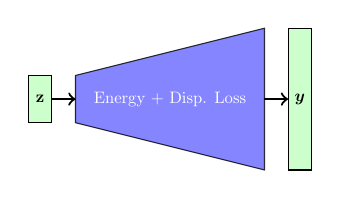
\begin{tikzpicture}[scale=0.6, every node/.style={scale=0.6}]
                          % Modal coordinate (z)
                          \draw[fill=green!20] (-3, 1) rectangle (-2.5,2);
                          \node at (-2.75, 1.5) {$\mathbf{z}$}; % Label inside the rectangle
                          % Displacement (y)
                          \draw[fill=green!20] (2.5,0) rectangle (3,3);
                          \node at (2.75, 1.5) {$\bm{y}$}; % Label inside the rectangle
                          % NN mapping
                          \draw[fill=blue!60,opacity=0.8] (-2,1) -- (2,-0) -- (2,3) -- (-2,2) -- cycle;
                          \node[white] at (0,1.5) {Energy + Disp. Loss};
                          % Arrow
                          \draw[thick,->] (-2.5, 1.5) -- (-2, 1.5);
                          \draw[thick,->] (2, 1.5) -- (2.5, 1.5);
                      \end{tikzpicture}
                \caption{Neural Modes architecture.}
                \label{fig:neural_modes_arch}
            \end{figure}
        \end{column}
    \end{columns}
\end{frame}

\begin{frame}{Training the Network}
    
    To apply our supervised approach, we follow these steps:
    \vspace{2em}
        \begin{enumerate}
            \item We use SOFA \cite{Faure_Duriez_Delingette_Allard_Gilles_Marchesseau_Talbot_Courtecuisse_Bousquet_Peterlik_2012} to solve Equation \ref{eq:static_problem} and generate a dataset of \( (\mathbf{z}, \bm{u}_{FEM}, E_{FEM}) \), where:
                        \begin{itemize}
                            \item \( \mathbf{z} \) are the input modal coordinates.
                            \item \( \bm{u}_{FEM} \) is the full nonlinear ground truth displacement.
                            \item \( E_{FEM} \) is the ground truth internal energy.
                        \end{itemize}
                        \item We \textbf{train the network} to minimize a loss function \(\mathcal{L}\) that combines supervised training with physics constraints, as defined in the loss function:
                        \[
                            \mathcal{L} = \alpha_1 \mathcal{L}_E + \alpha_2 \mathcal{L}_u + \gamma_1 \mathcal{L}_{ortho} + \gamma_2 \mathcal{L}_{BC}.
                        \]
        \end{enumerate}
\end{frame}

\begin{frame}[allowframebreaks]{The Loss Function}
    We define:
    \begin{equation*}
        \text{MSE} = \frac{1}{N} \sum_{i=1}^{N} (\bm{u}_{pred,i} - \bm{u}_{FEM,i})^2,
    \end{equation*}
     where \(N\) is the number of samples, and \(\bm{u}_{pred,i}, \bm{u}_{FEM,i}\) are the predicted and ground truth displacements.
    \begin{equation*}
    \mathcal{L}_{BC} = \frac{1}{N_{BC}} \sum_{i \in \mathcal{B}} \|\bm{u}_{pred,i} - \bm{u}_{BC,i}\|^2,
    \end{equation*}
    where \(N_{BC}\) is the number of boundary nodes, \(\mathcal{B}\) the set of boundary nodes \(\bm{u}_{pred,i}\) and \(\bm{u}_{BC,i}\) are the predicted and prescribed displacements at node \(i\).
    \vspace{7em}

    Our total loss function is a weighted sum of four components:
     \begin{equation*}
          \mathcal{L} = \textcolor{darkgreen}{\alpha_1 \mathcal{L}_E} + \textcolor{darkblue}{\alpha_2 \mathcal{L}_u} + \textcolor{darkorange}{\gamma_1 \mathcal{L}_{ortho}} + \textcolor{darkred}{\gamma_2 \mathcal{L}_{BC}}
     \end{equation*}
    \begin{description}
          \item[\textcolor{darkblue}{\(\mathcal{L}_u\) (Displacement Loss)}]
        \(\mathcal{L}_u = \text{MSE}(\bm{u}_{pred}, \bm{u}_{FEM})\).
          
          \item[\textcolor{darkgreen}{\(\mathcal{L}_E\) (Energy Loss)}] 
        \(\mathcal{L}_E = \text{MSE}(\log_{10}(E_{pred}), \log_{10}(E_{FEM})).\)
          
          \item[\textcolor{darkorange}{\(\mathcal{L}_{ortho}\) (Orthogonality Loss)}] A geometric constraint:
          \(
                \bm{l}^T \bm{y} = 0
          \)
          
          \item[\textcolor{darkred}{\(\mathcal{L}_{BC}\) (Boundary Loss)}] Penalizes violations of boundary conditions.
     \end{description}
     
\end{frame}

% \begin{frame}{Sampling Latent Space}
    
%     \begin{columns}[T]
%         \begin{column}{0.5\textwidth}
%             \textbf{Random Sampling}
            
%             Picking random \(\mathbf{z}\) from a uniform distribution often results in high-energy configurations.

%             \textbf{Structured Data Generation}
            
%             The supervised approach generates samples of \(\mathbf{z}\) that are:
%             \begin{itemize}
%                 \item Physically plausible.
%                 \item Cover the most important deformation patterns of the object.
%             \end{itemize}
            

%         \end{column}
        
%         \begin{column}{0.5\textwidth}

%             \begin{figure}
%                 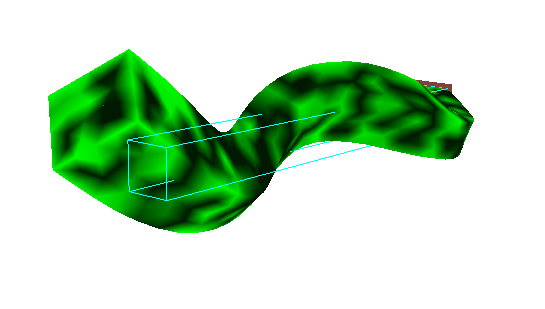
\includegraphics[width=\textwidth]{Images/z_random.png}
%                 \caption{Unnatural deformation from random sampling of high-frequency modes.}
%                 \label{fig:bad_sampling}
%             \end{figure}
           
%         \end{column}
%     \end{columns}

    
% \end{frame}

% \begin{frame}[allowframebreaks]{Data Generation}
%     \begin{itemize}
%         \item Ensure that the generated dataset represents \textbf{realistic deformations}.
%         \item Maintain a \textbf{balance} between the number of samples and the diversity of configurations.
%         \item Design a user-friendly and efficient pipeline for generating training data, especially for \textbf{complex geometries}.
%     \end{itemize}

    
%     \begin{block}{Modal Forces}
%         \begin{enumerate}
%             \item We linearize the system at rest to get the stiffness matrix \(\mathbb{K}\).
            
%             \item We perform an eigenvalue decomposition of \(\mathbb{K}\) to find the deformation modes \(\boldsymbol{\Phi}\).
            
%             \item We generate external forces as a linear combination of these modes:
%             \begin{equation*}
%                 \bm{f}^{ext} = \boldsymbol{\Phi} \bm{q}
%             \end{equation*}
%             where \(\bm{q}\) is a vector of modal force coefficients that we can control.
            
%             \item We apply these physically-grounded forces \(\bm{f}^{ext}\) to the \textbf{full nonlinear FEM solver} to compute the ground truth displacement \(\bm{u}_{FEM}\) and energy \(E_{FEM}\).
%         \end{enumerate}
%     \end{block}
    
% \end{frame}



% \begin{frame}{Dynamic Simulation}
    
%     Once trained, the Neural Modes network enables rapid dynamic simulations, by using L-BFGS to solve the optimization problem at each time step.
    
%     \begin{block}{Objective Function}
%         We find the next set of modal coordinates \(\mathbf{z}_{n+1}\) using:
        
%         \begin{equation}
%             \mathbf{z}_{n+1} = \underset{\mathbf{z}}{\argmin} \underbrace{\frac{1}{2h^2} \|\bm{n}(\mathbf{z}) - 2\bm{u}_n + \bm{u}_{n-1}\|_{\bm{M}}^2}_{\text{Inertial Term (Implicit Euler)}} + \underbrace{\mathcal{E}(\bm{n}(\mathbf{z}))}_{\text{Potential Energy}}
%         \end{equation}
%         where \(\bm{n}(\mathbf{z})\) is the full displacement predicted by our Neural Modes model and \(\mathcal{E}(\bm{n}(\mathbf{z}))\) the total potential energy of the system at time \(n\).
%     \end{block}
    
% \end{frame}


\begin{frame}{Numerical Results}
    
    We validate our method on two 3D geometries with soft tissue properties ($E = 10^6$ Pa, $\nu = 0.45$). Numerical results showed us that between \textbf{7 and 10 modes} are sufficient to capture the nonlinear deformation behavior of these objects.
    
    \begin{columns}[T]
        \begin{column}{0.45\textwidth}
            \textbf{1. Cantilever Beam}
            \begin{itemize}
                \item A classic structural benchmark.
                \item Simple deformation modes.
                \item Discretized with ~800 tetrahedral elements.
            \end{itemize}
        \end{column}
        
        \begin{column}{0.55\textwidth}
            \textbf{2. Stanford Bunny}
            \begin{itemize}
                \item A complex, realistic geometry.
                \item Irregular shape leads to complex nonlinear deformation.
                \item Discretized with ~22,000 tetrahedral elements.
            \end{itemize}
    
        \end{column}
    \end{columns}
\end{frame}

\begin{frame}{Meshes}
    \begin{columns}[T]
        \begin{column}{0.5\textwidth}
            \centering
            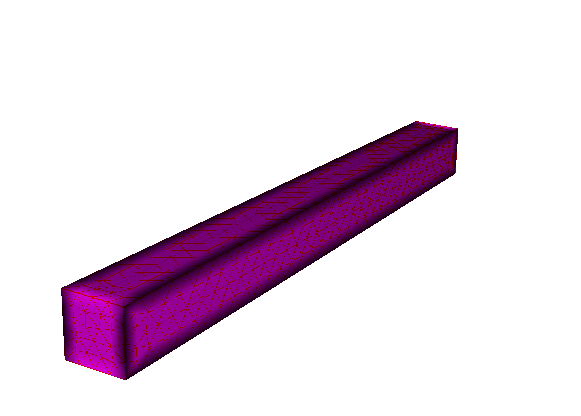
\includegraphics[width=0.8\textwidth]{Images/beam.png}
            \captionof{figure}{Cantilever Beam Mesh}
        \end{column}
        \begin{column}{0.5\textwidth}
            \centering
            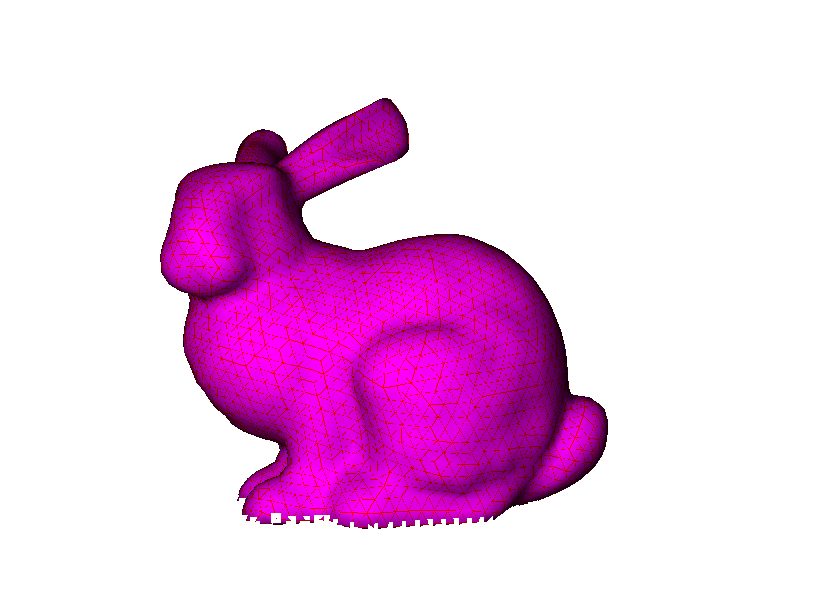
\includegraphics[width=0.8\textwidth]{Images/stanford_bunny.png}
            \captionof{figure}{Stanford Bunny Mesh \cite{bunny-mesh}}
        \end{column}
    \end{columns}
\end{frame}

\begin{frame}{Training}
    
    We trained our model using a supervised approach on datasets of 600 (beam) and 500 (bunny) FEM simulations.
    
\begin{columns}
    
    \begin{column}{0.5\textwidth}
            \textbf{Training Loss (Beam)}
            \begin{itemize}
                \item The model learns quickly, with the loss dropping significantly in the first few epochs.
                \item Training was stable over 200 epochs.
            \end{itemize}
    \end{column}
    \begin{column}{0.5\textwidth}
            \begin{figure}
                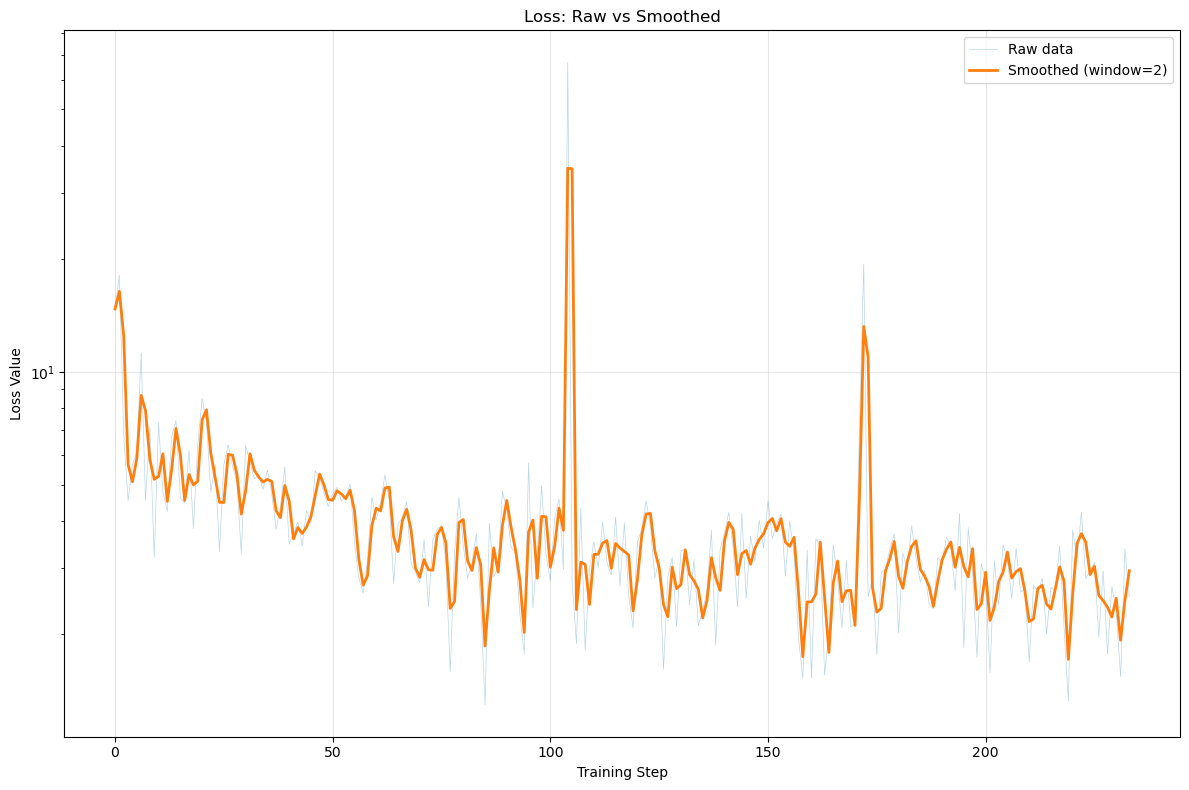
\includegraphics[width=\textwidth]{Images/training_loss_smoothed_logy.png}
                \caption{Total training loss.}
            \end{figure}

    \end{column}
        
\end{columns}

\end{frame}

\begin{frame}{Self-Supervised Approach}
    \begin{columns}[T]
        \begin{column}{0.4\textwidth}
            \vspace{5em}
            We tested the self-supervised approach, but it \textbf{failed} to achieve \textbf{sufficient accuracy} for our {problem}.  
    
        \end{column}
        
        \begin{column}{0.6\textwidth}
            \begin{figure}
                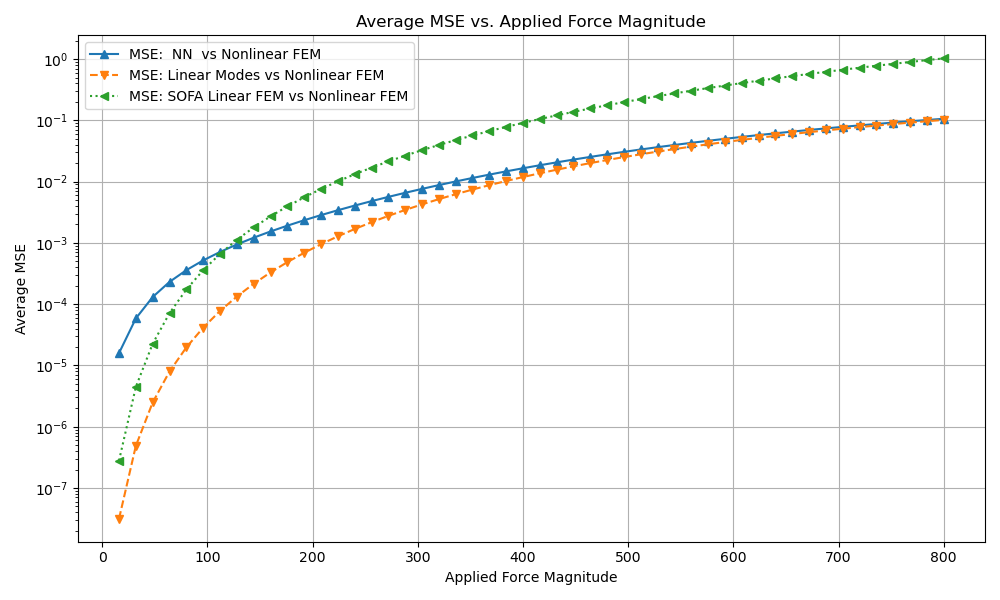
\includegraphics[width=\textwidth]{Images/self_supervised_mse.png}
                                \caption{\textcolor{darkblue}{Self-supervised} vs. \textcolor{darkorange}{Linear Modes}.}
            \end{figure}
        \end{column}
    \end{columns}
\end{frame}

\begin{frame}{Static Validation - 3D Beam}
    
    We obtain more than \textbf{one order of magnitude} improvement in accuracy over linear modes. Also for reference we included the \textcolor{darkgreen}{linear FEM} solution.
    \vspace{-1em}

    \begin{columns}[T]
        \begin{column}{0.5\textwidth}
   
            \begin{figure}
                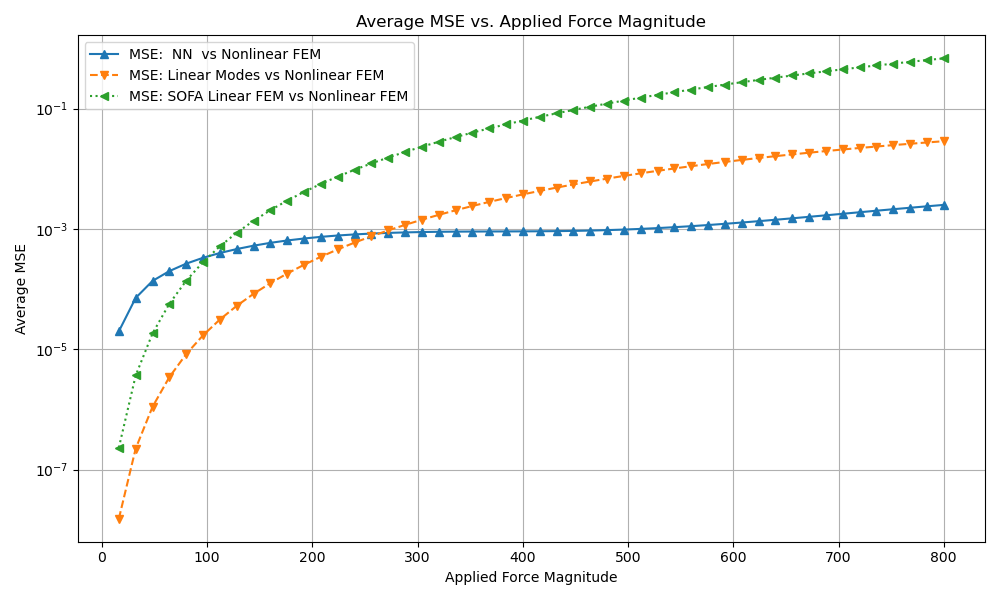
\includegraphics[width=\textwidth]{Images/beam_static_mse.png}
                \caption{MSE comparison between \textcolor{darkorange}{Linear Modes} and \textcolor{darkblue}{Neural Modes}.}
            \end{figure}
        \end{column}
        
        \begin{column}{0.5\textwidth}
            \begin{figure}
                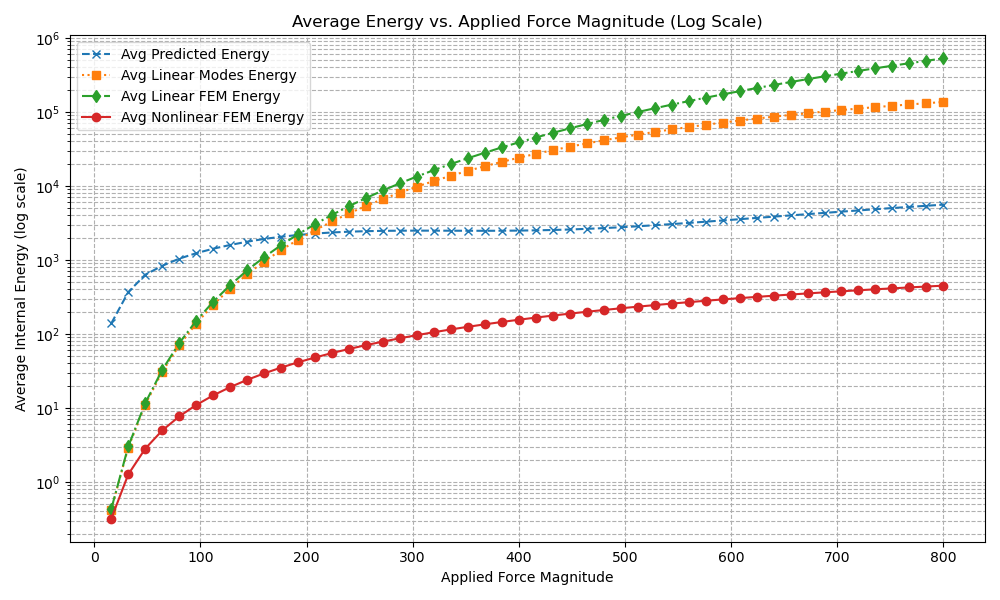
\includegraphics[width=\textwidth]{Images/beam_static_energy.png}
                \caption{Energy comparison. \textcolor{darkred}{Nonlinear FEM} is the ground truth.}
            \end{figure}
        \end{column}
    \end{columns}
\end{frame}

% \begin{frame}{Qualitative Results}
%     A visual result of the static validation for the beam and bunny geometries. We compare our \textcolor{magenta}{Neural Modes} and \textcolor{red}{Linear Modes} against the \textcolor{green}{Nonlinear FEM} solution. The \textcolor{blue}{Linear FEM} solution is also included for reference.
%     \begin{columns}[T]
%         \begin{column}{0.5\textwidth}            

%             \begin{figure}
%                 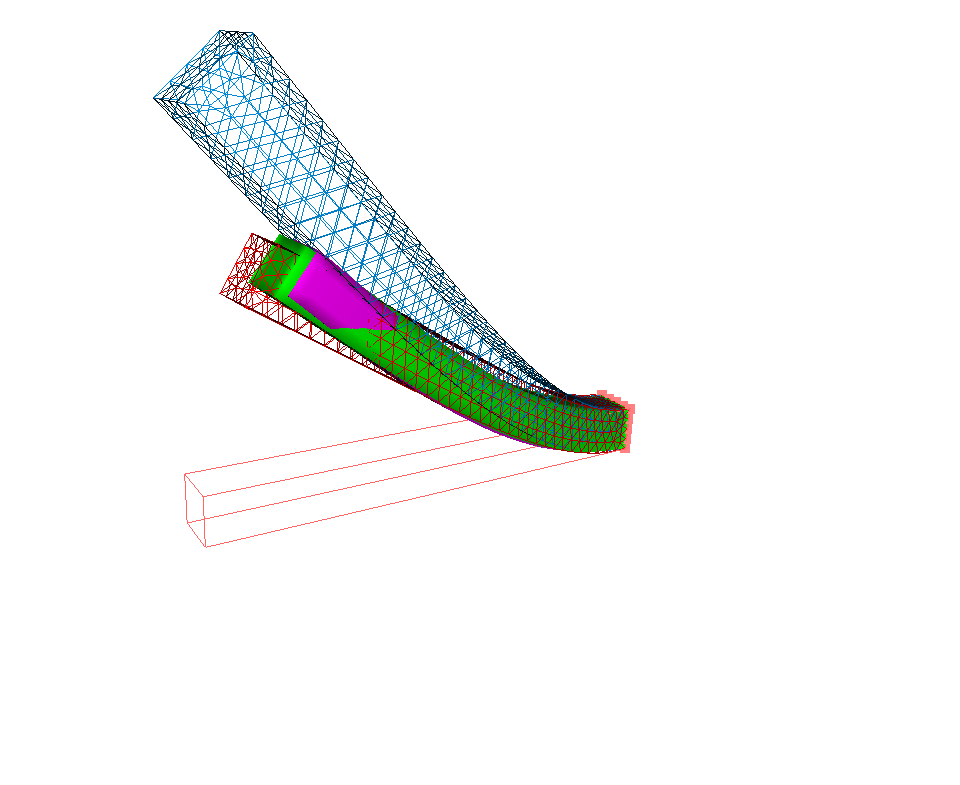
\includegraphics[width=0.7\textwidth]{Images/sofa_example_beam.png}
%                 \caption{Cantilever Beam}
%             \end{figure}
%         \end{column}
%         \begin{column}{0.5\textwidth}
%             \begin{figure}
%                 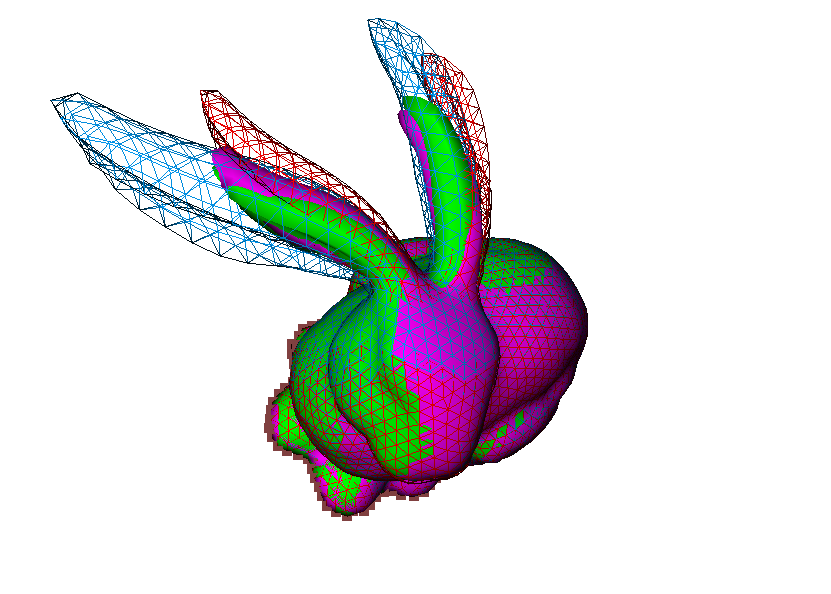
\includegraphics[width=0.8\textwidth]{Images/sofa_example_bunny.png}
%                 \caption{Stanford Bunny}
%             \end{figure}
%         \end{column}
%     \end{columns}
% \end{frame}

\begin{frame}{Static Validation - Stanford Bunny}
    
    On this complex geometry we obtain more than \textbf{one order of magnitude} improvement in accuracy over linear modes only in the range between 0-120 N. 
    \vspace{-1em}

    \begin{columns}[T]
        \begin{column}{0.5\textwidth}
   
            \begin{figure}
                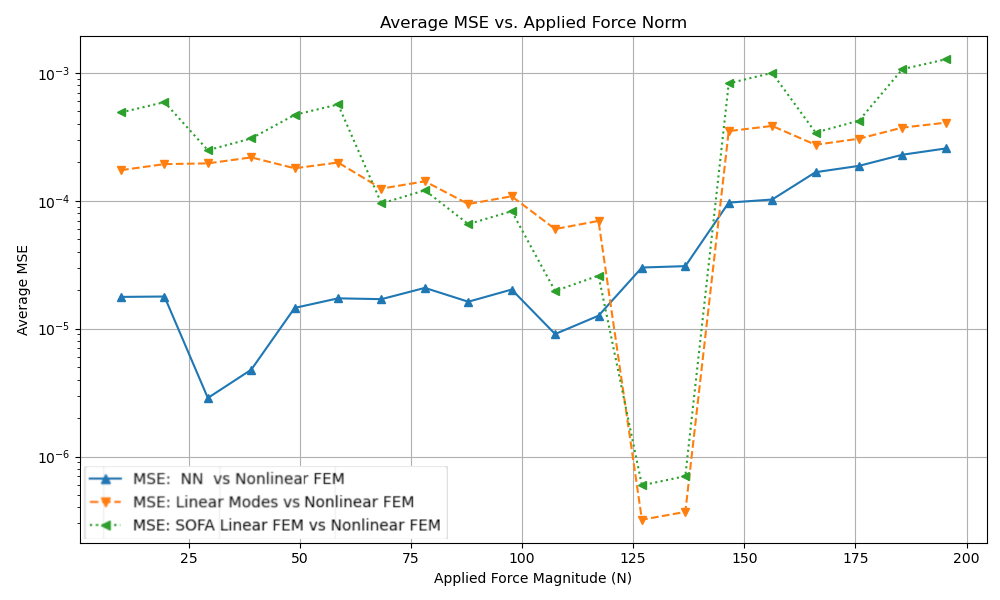
\includegraphics[width=\textwidth]{Images/bunny_static_mse.png}
                \caption{MSE comparison between \textcolor{darkorange}{Linear Modes} and \textcolor{darkblue}{Neural Modes}.}
            \end{figure}
        \end{column}
        
        \begin{column}{0.5\textwidth}
            \begin{figure}
                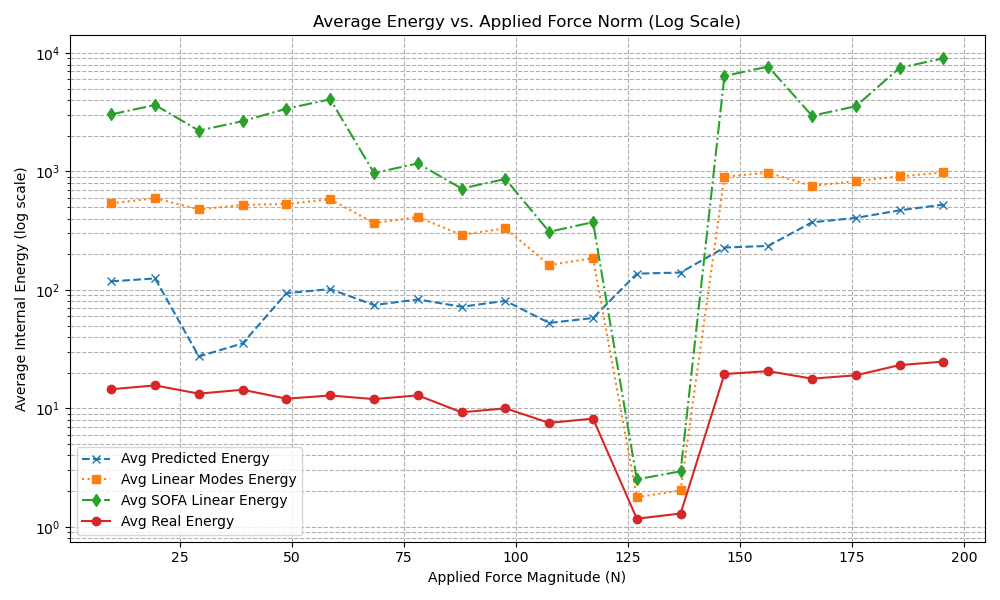
\includegraphics[width=\textwidth]{Images/bunny_static_energy.png}
                \caption{Energy comparison. \textcolor{darkred}{Nonlinear FEM} is the ground truth.}
            \end{figure}
        \end{column}
    \end{columns}
\end{frame}

\begin{frame}{Interpretability}
    \begin{columns}[T]
        \begin{column}{0.3\textwidth}
            \vspace{3em}
   The framework allows us to \textbf{visualize the corrections} for each mode, which is a significant \textbf{advantage} over ``black-box'' neural networks.
        \end{column}
        \begin{column}{0.7\textwidth}
            \begin{figure}
                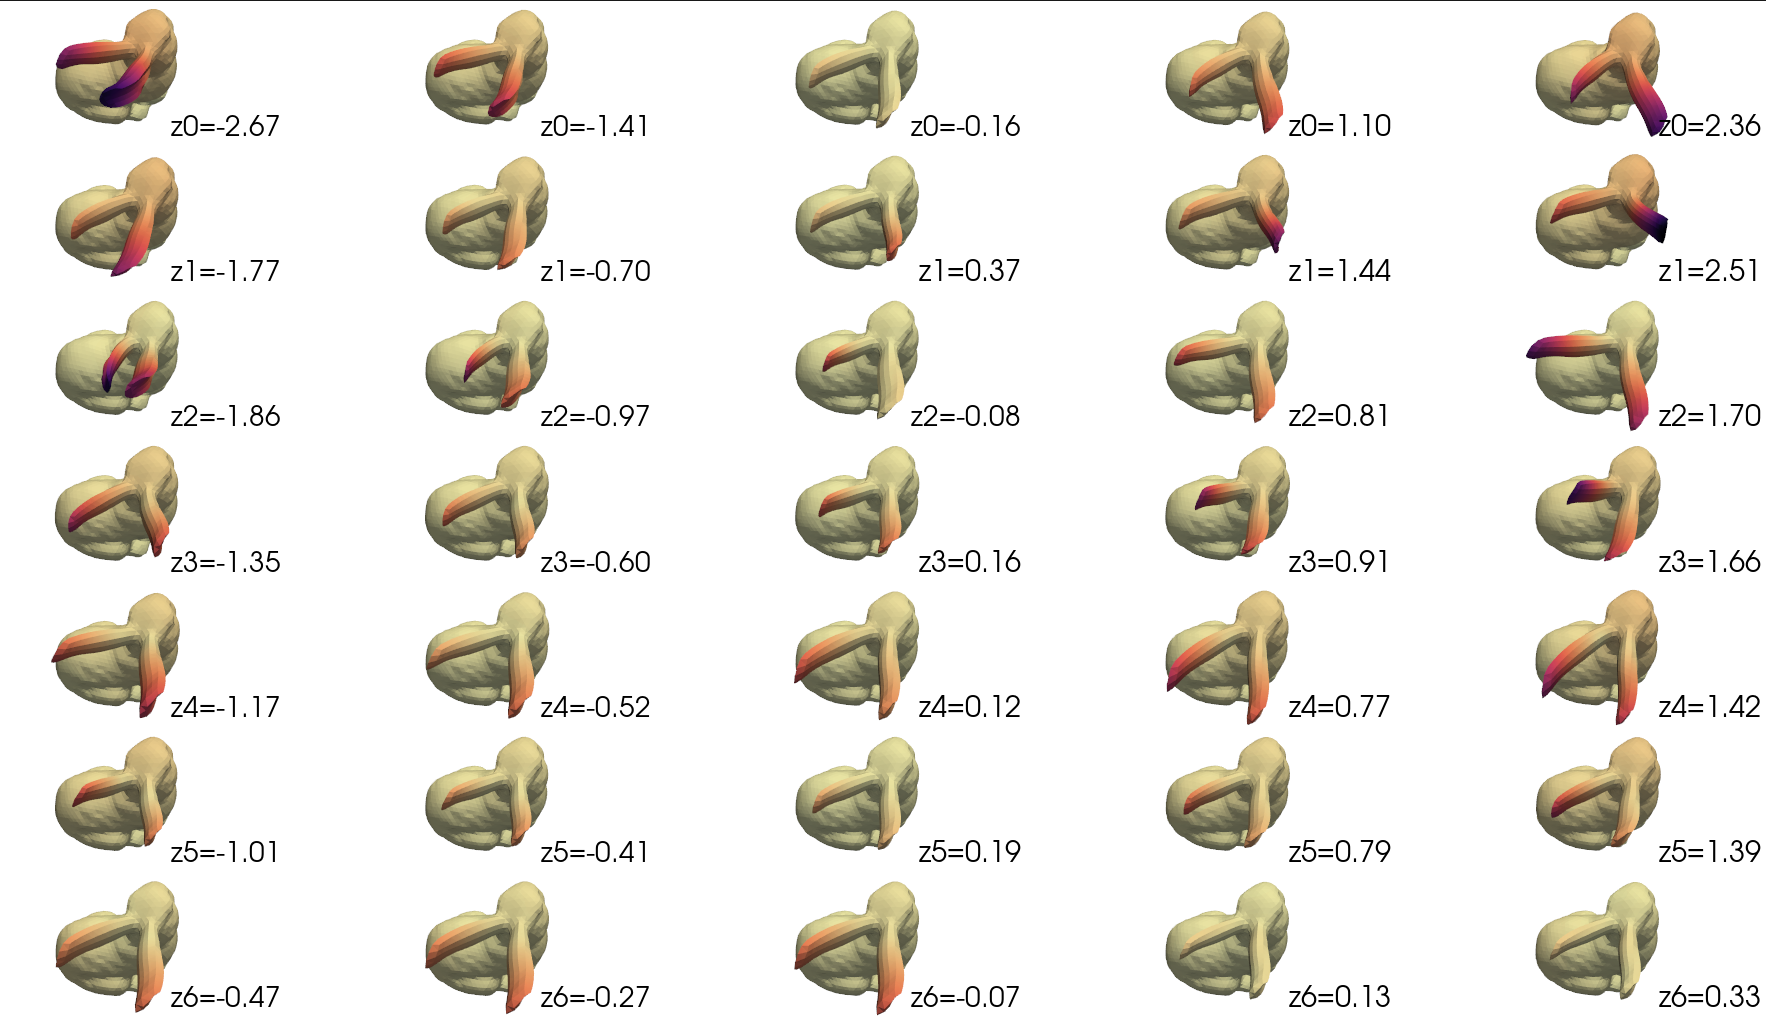
\includegraphics[width=0.8\textwidth]{Images/latent_space_viz.png}
                \caption{Visualization of the learned corrections for the 7 modes of the Stanford Bunny.}
            \end{figure}
        \end{column}
    \end{columns}
\end{frame}
\begin{frame}{Dynamic Validation}
    \begin{columns}[T]
        \begin{column}{0.5\textwidth}
            \textbf{Validation Process}
            \begin{itemize}
                \item We let SOFA solve the first 70 timesteps of the dynamic problem (see Equation \ref{eq:dynamic_problem}).
                \item After 70 timesteps, we switch to the dynamic update method (see Equation \ref{eq:dynamic_update}).
                \item The error is computed with respect to the FEM solver for the remaining timesteps.
            \end{itemize}
        \end{column}
        \begin{column}{0.5\textwidth}
            \textbf{Dynamic Problem}
            \begin{equation}
                \begin{cases}
                    \rho \frac{\partial^2 \bm{u}}{\partial t^2} - \nabla_X \cdot \bm{P} = \bm{b} \quad \text{in} \quad \Omega, \\
                    \bm{u} = \bm{u}_D \quad \text{on} \quad \Gamma_D, \\
                    \bm{P} \cdot \bm{N} = \bm{t} \quad \text{on} \quad \Gamma_N.
                \end{cases}
                \label{eq:dynamic_problem}
            \end{equation}
            Here, \(\rho\) is density, and the rest of the notation is as before.
        \end{column}
    \end{columns}
\end{frame}





\begin{frame}{Dynamic Validation}
    
    We let the model predict almost \textbf{200 time steps} of dynamic simulation, and the results show that while the displacement accuracy drifts over time, the internal energy remains \textbf{stable}.
    \vspace{-1em}
        
    \begin{columns}[T]
        \begin{column}{0.5\textwidth}
            \begin{figure}
                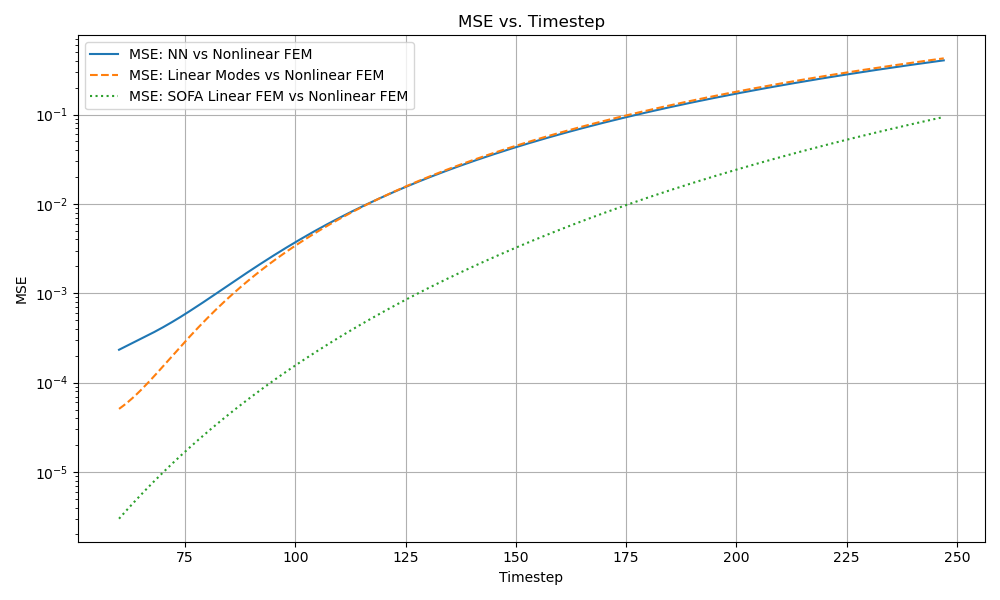
\includegraphics[width=\textwidth]{Images/beam_dynamic_mse.png}
                                \caption{\textcolor{darkblue}{Neural Modes} vs. \textcolor{darkorange}{Linear Modes} displacement accuracy over time.}
            \end{figure}
        \end{column}
        
        \begin{column}{0.5\textwidth}
            \begin{figure}
                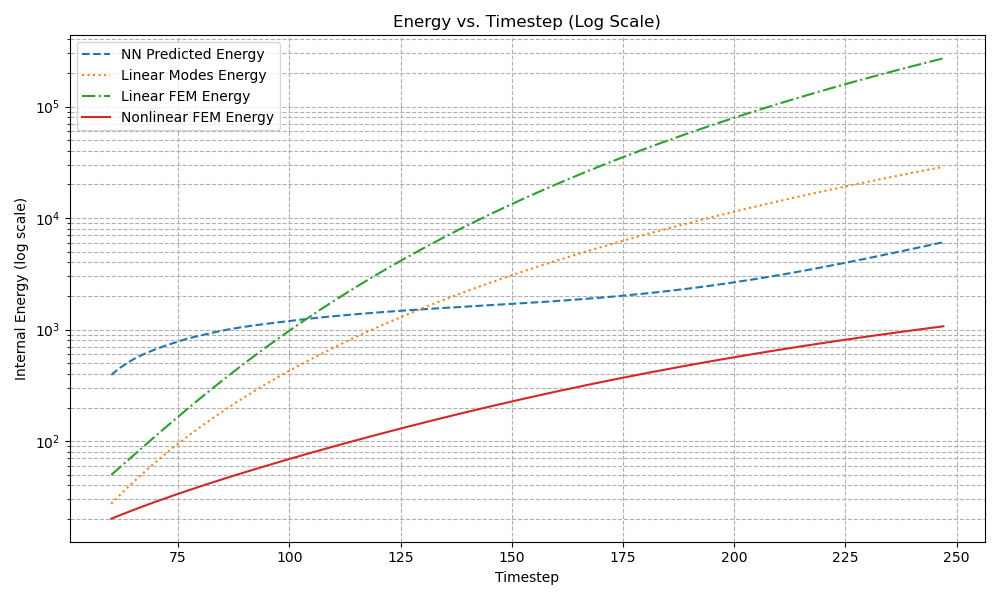
\includegraphics[width=\textwidth]{Images/beam_dynamic_energy.png}
                \caption{\textcolor{darkblue}{Neural Modes} vs. \textcolor{darkorange}{Linear Modes} internal energy over time.}
            \end{figure}
        \end{column}
    \end{columns}
\end{frame}

\begin{frame}{Conclusions}
    
    \begin{itemize}
        \item A data-free, self-supervised approach was insufficient for our problem, while a \textbf{supervised training} returned excellent results.
        
        \item  In static tests, our Neural Modes model is up to an \textbf{order of magnitude more accurate} than linear models for large, nonlinear deformations.
   
        
        \item In dynamic simulations, while positional accuracy eventually drifts, our model maintains \textbf{stable and realistic internal energy}
        \item The framework is \textbf{interpretable}, allowing us to visualize the learned nonlinear corrections.
    \end{itemize}
\end{frame}


\begin{frame}{Limitations and Future Work}
    
    One of the current limitations of our approach is the dynamic accuracy.

    A promising future direction to address this limitation is to adopt a \textbf{fully reduced dynamics approach}. Projecting the system matrices onto the modal basis:
    \[
        \left[M\right] = \left[\Phi\right]^T M \left[\Phi\right], \quad \left[K\right] = \left[\Phi\right]^T K \left[\Phi\right].
    \]
Then one would solve:
    \[
        \left[{M}\right] \ddot{\mathbf{q}} + \left[{K}\right] \mathbf{q} = \mathbf{f}.
    \]
    This approach could enable more stable numerical integration and significantly improve long-term accuracy.

\end{frame}

%closing frame 
\begin{frame} %
    \centering
    \Huge Thank you for your attention! 
    \vspace{1em}
    
\end{frame}

%bibliography
\begin{frame}[allowframebreaks]{References}
    \printbibliography[heading=none]
\end{frame}


\end{document}

